\RequirePackage{fix-cm,cmap}

\documentclass[
fontsize=11pt,
paper=a4,
abstract=true,
numbers=noenddot,
listof=totoc,
bibliography=totoc,
twoside,
open=right,
cleardoublepage=plain,
parskip=half+, % comment this out if you do not want an empty half line between paragraphs, but please read the KomaScript Guide and search for parskip (around page 82): ftp://ftp.dante.de/pub/tex/macros/latex/contrib/koma-script/scrguide.pdf
BCOR=1cm, % Bindekorrektur: Change this accordingly, also read the KomaScript Guide! Make sure you read the guide.
]{scrreprt}

\setcounter{tocdepth}{3}  % Inhaltsverzeichnis bis Subsubsection
\setcounter{secnumdepth}{3} % Nummerierung bis Subsubsection

% General stuff
\usepackage[utf8]{inputenc} % CHANGE HERE IF NECESSARY
\usepackage[T1]{fontenc}
\usepackage[ngerman, english]{babel} % last language given is used (here: english)
\usepackage{lmodern}
%\usepackage{microtype}
\usepackage{ifpdf}
\usepackage{ifthen}

% Set date here 
%\day=6 \month=6 \year=2012

% Set name and title
\author{\textbf{Shashank Kanakapura Srivatsa}\\
University of Paderborn\\
Paderborn, Germany\\
srivatsa@mail.uni-paderborn.de}
\title{HTTP Desync Attacks: Smashing into the Cell
	Next Door}
\date{\today}

%%%%%% %%%%%%

% Load packages ...

% Corporate Design
\usepackage{eso-pic}
\usepackage{color}
% Comment out if the RUB fonts are installed
% Link: https://noc.rub.de/~jobsanzl/latex/rubtexfonts-0.4.tar.gz
%\usepackage{rubfonts2009} 
\newcommand{\setrubfontnormal}[1]{\fontfamily{rubscala}\fontsize{#1}{1}\selectfont}
\newcommand{\setrubfontextra}[1]{\fontfamily{rubflama}\fontsize{#1}{1}\selectfont}
\definecolor{rubgreen}{cmyk}{0.5,0,1,0}
\definecolor{rubblue}{cmyk}{1,0.5,0,0.6}

% Figures
\usepackage{graphicx}
\usepackage{subfig}
\usepackage{placeins}

% Tables
\usepackage{booktabs}
\usepackage{marvosym}
\usepackage{multirow}

% Math stuff and units
\usepackage{latexsym,amsmath, amssymb, amsfonts, upgreek}
\usepackage{siunitx}
\newcommand{\mathup}{\mathrm}

% Glossary
\usepackage[nonumberlist, acronym, toc]{glossaries}

% Enable quotes by \enquote{}
\usepackage[babel,english=american, german=quotes]{csquotes}

% Necessary for frontpage, allows to create automata and fancy graphics
\usepackage{tikz}

% Protocols and bytefields
\usepackage{protocol}
\usepackage{bytefield}

% Source code listings
\newcommand{\code}[1]{\texttt{#1}}
\definecolor{colIdentifier}{rgb}{0,0,0}
\definecolor{colComments}{rgb}{0.5,0.5,0.5}
\definecolor{colKeys}{rgb}{0,0,1}
\definecolor{colString}{rgb}{0,0.6,0}

\usepackage{caption}
\usepackage{listings}
\lstset{%
	float=hbp,%
	basicstyle=\ttfamily\scriptsize, %
	identifierstyle=\color{colIdentifier}, %
	keywordstyle=\color{colKeys}, %
	stringstyle=\color{colString}, %
	commentstyle=\color{colComments}, %
	columns=flexible, %
	tabsize=2, %
	aboveskip={1.5\baselineskip}, %
	frame=single, %
	extendedchars=true, %
	showspaces=false, %
	showstringspaces=false, %
	numberstyle=\tiny, %
	breaklines=true, %
	backgroundcolor=, %
	breakautoindent=true, %
	captionpos=b%
}

% Algorithms
\usepackage[ruled, vlined, linesnumbered,algochapter,algo2e]{algorithm2e}

% Format page foot and header
\usepackage{scrpage2}
\clearscrheadings
\clearscrheadfoot
\automark[section]{chapter}
\ohead{\pagemark}
\ihead{\headmark}
\pagestyle{scrheadings}

%% use some standards for mathematical expressions:
\newcommand{\red}{{\rm red}}
\newtheorem{theorem}{Theorem}[section]
\newtheorem{lemma}[theorem]{Lemma}
\newtheorem{proposition}[theorem]{Proposition}
\newtheorem{corollary}[theorem]{Corollary}
% \newtheorem{definition}[theorem]{Definition}
\newtheorem{algorithm}[theorem]{Algorithm}
\newenvironment{example}{\begin{quote}{\bf Example:}}{\end{quote}}

% BIBTEX, http://mirrors.ctan.org/biblio/bibtex/contrib/babelbib/babelbib.pdf
\usepackage{babelbib}
\usepackage{url}
\def\UrlBreaks{\do\/\do-}

% \setbibpreamble{{\large Seitenzahlen, auf denen ein Eintrag referenziert wird, werden am Ende eines jeden Eintrags angegeben.}\newline} % Wegen der pagebackref-Option des hyperref-Packets, wird vielen nicht direkt klar was das soll http://projekte.dante.de/DanteFAQ/Verzeichnisse#16

% gray definition boxes, that whay you'll find them in the text
\usepackage{shadethm}
\newshadetheorem{sthm}[figure]{Definition}
\newenvironment{definition}[1][]{
   \definecolor{shadethmcolor}{rgb}{.9,.9,.9}
   \begin{sthm}[#1]
 }{\end{sthm}}

% experimental
%\usepackage{scrhack}

% Hyperlinks and menu for your document
\usepackage[breaklinks,hyperindex,colorlinks,anchorcolor=black,citecolor=black,filecolor=black,linkcolor=black,menucolor=black,urlcolor=black,pdftex]{hyperref} % pagebackref: Add page number to the references where they can be found
% DO NOT LOAD ANY OF YOUR PACKAGES BEYOND THIS PACKAGE

\makeatletter
\AtBeginDocument{
 \hypersetup{
   pdftitle = {\@title},
   pdfauthor = {\@author},
   pdfsubject={\@title},
   pdfkeywords={SAML, add more}, % CHANGE HERE
%    unicode={true},
 }
}
\makeatother

% Use the same counter for tables and figures
\makeatletter
\AtBeginDocument{
\let\c@table\c@figure
\let\c@lstlisting\c@table
\let\c@algocf\c@lstlisting
}
\makeatother

\ifpdf
	\hypersetup{linktocpage=false} 	% false=links are section names, true=links are page numbers, IMPORTANT: in dvi2ps mode, 'true' is required!
\else
	\hypersetup{linktocpage=true} 		% false=links are section names, true=links are page numbers, IMPORTANT: in dvi2ps mode, 'true' is required!
	\usepackage[hyphenbreaks]{breakurl}
\fi


\usepackage{cite}
\usepackage{amsmath,amssymb,amsfonts}
\usepackage{algorithmic}
\usepackage{graphicx}
\usepackage{textcomp}
\usepackage{xcolor}

\begin{document}

%% title page --- made out of expressions defined above
% Hintergrund-Makro
\newcommand\BackgroundPic{
\put(0,0){
\parbox[b][\paperheight]{\paperwidth}{%
\vfill
\centering

\includegraphics[width=\paperwidth,height=\paperheight]{images/images_front}%
\vfill
}}}

\AddToShipoutPicture*{\BackgroundPic}
\begin{titlepage}
\makeatletter

\enlargethispage{3cm}

\begin{minipage}[b]{1\linewidth}
	\sffamily
	
\includegraphics[scale=0.5]{images/images_upb_logo}
  	\vspace*{8cm}
  	
	\textbf{\LARGE {\@title}}\\
  
	\Large{\@author}\\
	
% 	\vspace*{35mm}
	\vspace{4cm}
	\normalsize{
	Seminar report\@~~--~~\@date\@.\\
	System Security Group.\\}
	\newline
	\normalsize{
	\begin{tabular}{@{}ll@{}}
	Supervisors: 	& \textbf{Prof.~Dr-Ing.~Juraj Somorovsky}\\
					& University of Paderborn\\
					& Paderborn, Germany\\
					& juraj.somorovsky@upb.de
	\end{tabular}
	}
\end{minipage}


\makeatother
\end{titlepage}
\ClearShipoutPicture

\begin{abstract}
	Internet has become an integral part of the modern world and it is extremely difficult to imagine a world without internet. One of the most significant activity on the internet is exchange of data between computers, generally referred to as Clients and Servers. There are a huge number of formats in which the data can be transferred over internet and many new formats are being introduced. To organize and govern such data transfers, several protocols have been defined by organisations. One of the prominent protocol is Hyper Text Transfer Protocol(HTTP), where a Client submits a request to the Server over the internet and the Server responds to the Client with approriate data or message.\\
	Like several other protocols, HTTP also contains some vulnerabilities which can be exploited by malicious attackers and thus it becomes extremely necessary to identify such vulnerabilities. Security experts or \textit{White hat hackers} help to identify vulnerabilities present in protocols such as HTTP and notify the concerning organisations or individuals about the same. This helps to fix the vulnerabilities present and thus prevent information leakage. There are several vulnerabilities that have been identified in the past and many of these problems are already addressed. In this report, we talk about a relatively new technique known as 'HTTP Desync Attack' which is developed to exploit the vulnerability in HTTP protocol. In this technique, the attacker tricks the Server into believing that the malicious request is actually a part of a normal user`s request and thus allows the attacker to gain control over the request. This report reviews HTTP Desync Attacks in detail and further evaluates it to understand the pros and cons of the technique. 
	
\end{abstract}


\cleardoublepage

\pagenumbering{arabic} %switches to arabic numbers for the rest of the text
\chapter{Introduction}

As the world around us is developing rapidly, many things are moving online. As organisations and individuals are increasingly preferring new-age inventions such as Cloud Storage, IoT devices, Online Banking etc., these technologies require one basic thing - Internet. Internet has become an integral part of our daily lives. In its early years, internet was only used for crucial transactions inside corporate and government organisations, and for mail exchanges. However, over the last two decades it has completely taken over the lives of a common individual. Approximately 60\% of the world`s population depends on internet for day-to-day activities \cite{b16}. 

With such advancements, the need for internet security is more than ever and organisations are investing a substantial part of their revenue on security\cite{b2}. Even though we try to reduce security related incidents, attackers are inventing clever ways to bypass existing security protocols. According to a reputed corporate organisation, there has been a 11\% increase in security breaches since 2018 and 67\% since 2014\cite{b3}. It is estimated that hackers attack every 39 seconds, on an average 2,244 times a day\cite{b4}. If an attacker is able to control or snoop on the data being exchanged over the internet, it can be used for malicious purposes. It can contain personal information of a person or an organisation, confidential data of governments and organisations, financial data and so on.

Internet security protocols and standards help in tackling the above stated problems. Even though attackers have found ways to exploit the vulnerabilities in the existing protocols governing the internet, experts and researchers are constantly improving these protocols to better equip the world in tackling this menace.  

Some of the popular security protocols are Secure File Transfer Protocol (SFTP), HyperText Transfer Protocol (HTTP), Secure Socket Layer (SSL) and so on. In this seminar we consider HTTP. HTTP is a protocol mainly used for data exchanges between computer systems. It is usually used in a Client-Server environment, where the Client sends a request to the Server and the Server responds with data, resource or message. A request from the Client or a response from the Server can contain sensitive information such as credentials, financial data, confidential files belonging to an organisation or a government, personal information and so on. If an attacker intercepts these information it could put the victim at risk.  

HTTP has been constantly improved and has become an important protocol to secure the data that is transmitted over the internet. However, as the growth of internet increases the need for securing these data transfers also increases with it. Like any other security protocol, even HTTP has vulnerabilities which are being exploited by attackers. There are several techniques for such exploits. Here we consider a relatively new technique known as 'HTTP Desync Attack' with which the attacker can create havoc on the target systems. The basic idea of this technique was first document by Watchfire in 2005\cite{b5}. This technique was however recently brought to the limelight by the works of by James Kettle\cite{b6}. Using this technique, the attacker can introduce carefully crafted malicious request through the front-end. Consider a front-end application which communicates with a back-end server.  Whenever a HTTP request is created, it includes HTTP Header and HTTP Body. The headers are sent to the servers for synchronisation. In a real setup, there are streams of requests coming from a large set of users. Hence it is important for the server to know where a request starts and ends. These HTTP Headers help the server to identify such crucial points and thus help in synchronisation. The attacker can however utilize the information present in the HTTP Header to cleverly trick the server and desynchronise the system. The corressponding malicious data is thus treated as part of a legitimate user`s request. This results in attacker gaining control of the victim user`s request. We will elaborately discuss about the details of this technique in the further parts of thos report and will also look at some case studies. 

The organisation of this report is as follows - In Chapter 2 we introduce some background concepts which might be required to understand the technique we discuss. Chapter 3 describes the problem and in Chapter 4 we elaborately discuss the details of this technique. In Chapater 5 we look at some real case studies to better understand the technique and Chapter 6 further evaluates the technique based on all the information discussed till then. We finally give a connclusion. 




\chapter{Background}
\section{HTTP} 
Hyper Text Transfer Protocol(HTTP) \cite{b1} is a stateless application layer protocol meant for distributed, collaborative, hypertext information systems. The exchange of data between a client and a server is governed by HTTP. A client sends a HTTP request which can contain standard as well as user's custom data together. The client receives this request and decodes the same. Based on the request the server decides to either perform an action or send data back to the client which can contain requested information or server messages.  

\section{HTTP 1.1}
HTTP 1.1 \cite{b1} is an improvised version of HTTP which succeeds the version HTTP 1.0. This version includes several improvements, few of which are :
\begin{itemize}
	\item support for keep-alive feature where a connection can be re-used.
	\item pipelining
	\item chunked responses
\end{itemize} 

\section{HTTP Request}
\cite{b7}A HTTP Request is a message sent by the client, to the server, to invoke an action at the server side.

\section{HTTP Response}
\cite{b7}A HTTP Response is a message sent back by the server, to the client, which contains the requested information, resource and status code. 

\section{HTTP Request Methods}
\cite{b8}These are verbs which specify the action that has to be performed by the server. The popular ones are :
\begin{itemize}
	\item GET : To request data from the resource.
	\item POST : To submit information to a resource. 
	\item PUT : To submit information to a resource but replaces the existing information. 
	\item DELETE : Deletes the specified resource. 
\end{itemize}

\section{HTTP Headers}
Headers contain meta-deta which corressponds to the request, request method and the information being communicated. 
\section{HTTP Body}
It is the information being transmitted and the response message received.

\chapter{Problem Statement}
HTTP/1.1 was first documented in RFC 2068 \cite{b9} and since its inception, it supports sending multiple HTTP requests over the same TCP or SSL/TLS socket. The HTTP requests are sent back to back and the server uses the HTTP headers to identify where a request ends and the subsequent request starts. 
\begin{figure}
	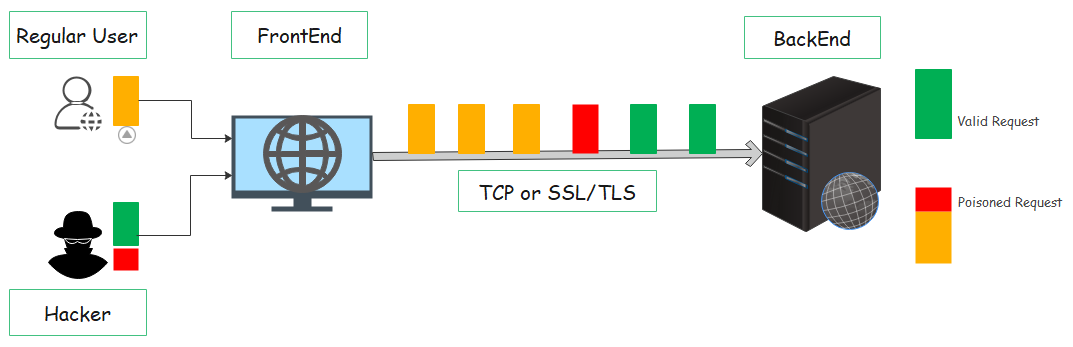
\includegraphics[width=4cm, keepaspectratio]{images/HTTP_Desync}
	\caption{HTTP Desync Attack}
	\label{fig:HTTP Desync Attack}
\end{figure}

\chapter{Core Concepts}
The HTTP Header fields mainly used to carry out desynchronization attacks are \textsc{Content-Length} and \textsc{Transfer-Encoding: chunked}. There are two combinations possible : 
\section{Using two Content-Length header fields:}
	This technique is very simple but is rarely effective as most of the modern systems are designed to selectively reject any requests with multiple \textsc{Content-Length} headers.\\
	Below is an example HTTP request, referenced from \cite{b6}:
	\begin{verbatim}
	POST / HTTP/1.1
	Host: example.com
	Content-Length: 6
	Content-Length: 5
	\end{verbatim}
\section{Using combination of Content-Length and Transfer-Encoding: chunked header fields:}This technique can be used to realize practical attacks in real environments. 
	Below is an example request, referenced from \cite{b6}:
	\begin{verbatim}
	POST / HTTP/1.1
	Host: example.com
	Content-Length: 3
	Transfer-Encoding: chunked
	\end{verbatim}
	This technique is valid as per the specifications in RFC 2616\cite{b10} which states : \\
	\textit{"If a message is received with both a Transfer-Encoding header field and a Content-Length header field, the latter MUST be ignored".}\\
	The core idea here is to hide the \textsc{Transfer-Encoding:chunked} header field from atleast one system in a chain of systems. It will make sure that the \textsc{Content-Length} header is used as a fallback and this will allow us to desynchronize the whole system.

We can explain this technique using two simple examples : 
\begin{itemize}
	\item Take a look at the example in figure \ref{fig:Frontend} which is referenced from \cite{b6}:
	If the frontend doesn't support chunked encoding, this kind of a request can be sent. Every chunk is constituted chunk size, followed by a new line and then the contents of the chunk. As frontend ignores chunked encoding, the backend considers the \textsc{Content-Length} header, appending the malicious message to the next request and thus desynchronizing the system.
\end{itemize}

\begin{figure}
	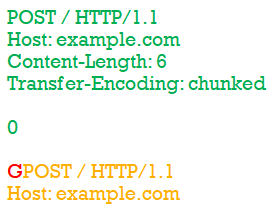
\includegraphics{images/Frontend}
	\caption{Frontend}
	\label{fig:Frontend}
\end{figure} 

\begin{itemize}
	\item Take a look at the example in figure \ref{fig:Backend} which is referenced from \cite{b6}: This kind of request is helpful when the backend ignores chunked encoding. The logic works same as described for frontend.
\end{itemize}
\begin{figure}
	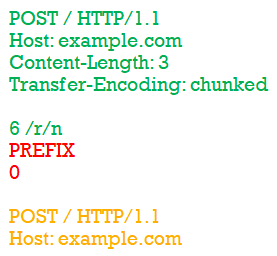
\includegraphics{images/Backend}
	\caption{Backend}
	\label{fig:Backend}
\end{figure}

Further complex desynchronizations can be achieved by carefully hiding the \textsc{Transfer-Encoding} header field or making it harder to detect. 

\chapter{Approach}
The author in \cite{b6} proposes a step approach to carry out desynchronization attacks. Figure \ref{fig:Phases} shows the phases of a desynchronization attack or request smuggling. Before explaining each of the phases in request smuggling, we need to observe that there are four possible configurations between the systems:
\begin{itemize}
	\item \textbf{CL.CL : } Both the frontend and backend servers use \textsc{Content-Length} header. As we have already seen, this configuration doesn't help in realizing attacks on practical modern systems. 
	\item \textbf{CL.TE : } Frontend server uses \textsc{Content-Length} header field and Backend server uses \textsc{Transfer-Encoding} header field. 
	\item \textbf{TE.CL : } Frontend server uses \textsc{Transfer-Encoding} header field and Backend server uses \textsc{Content-Length} header field.
	\item \textbf{TE.TE : } Both the frontend and backend servers use \textsc{Transfer-Encoding} header field.
\end{itemize}
\begin{figure}
	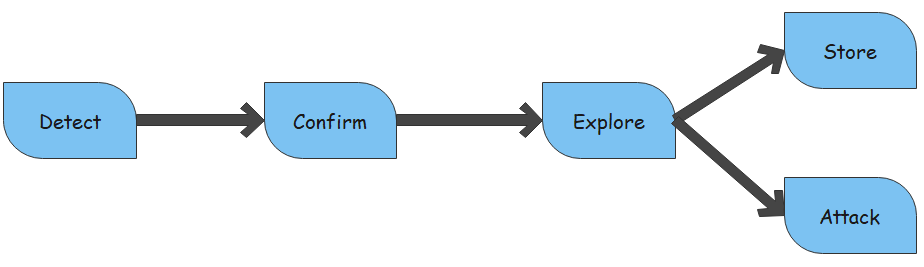
\includegraphics[width=14cm]{images/Phases}
	\caption{Phases of request smuggling}
	\label{fig:Phases}
\end{figure}
We will now look at each of the phases in detail:
\section{Detect}
The first step is to detect when a server will be vulnerable to desynchronization. A simple method here is to send a request with malicious data and poison the backend. Subsequent back to back requests are then sent to the same backend server. If the subsequent requests get an unexpected or erroneous response, we can assume that the response was due to the malicious prefix sent with the first request.  \\
However this technique isn't as simple as it looks and has a major drawback. When we try to detect desynchronization vulnerabilities in a website with a live traffic, there are numerous requests coming from many different users. If there is a normal user's request between our first malicious request and the subsequent follow up requests we send, it causes an error to the normal user and doesn't affect the follow up requests. Hence we cannot detect the vulnerability as we will not be able to observe the responses. \\
To tackle this problem, the author in \cite{b6} proposes an approach which uses server time-outs to the attacker's advantage. The configuration \textbf{CL.CL} and \textbf{TE.TE} cannot be used here for our advantage. However, \textbf{CL.TE} and \textbf{TE.CL} can be used. \\

\begin{figure}
	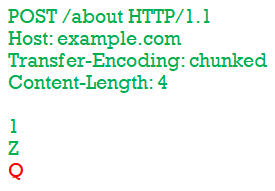
\includegraphics{images/CL.TE}
	\caption{CL.TE}
	\label{fig:CL.TE}
\end{figure}

\begin{figure}
	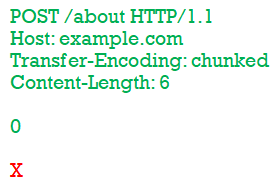
\includegraphics{images/TE.CL}
	\caption{TE.CL}
	\label{fig:TE.CL}
\end{figure}

\subsection{Case Study for \textit{Detect} phase}
Consider the example for \textbf{CL.TE} in Figure \ref{fig:CL.TE} (Referenced from \cite{b6}). As \textcolor{myred}{Q} is not a valid chunk size, the frontend will forward only the information highlighted in \textcolor{mygreen}{green} and the backend will timeout waiting for next valid chunk size. \\
Consider another example for \textbf{TE.CL} in figure \ref{fig:TE.CL}(Referenced from \cite{b6}). In this request, \textcolor{mygreen}{0} is explicitly placed to force the server into considering it as the \textit{terminating chunk}. As a result, the server will timeout waiting for \textcolor{myred}{X}.\\
These observable delays are sufficient to infer that the system has a vulnerability for request smuggling.\\

\section{Confirm}
Once we are sure that a system is vulnerable for request smuggling, we need to confirm the same with the help of responses that serve as visible proofs. The technique to get such confirmation is by poisoning the backend socket. The follow-up requests we send will fall victim to the earlier poisoning and will return a response to visibly prove that the vulnerability is present. One hindrance here is disconnection. If the first request causes an error, the backend system may have been designed to drop the connection and associated buffers. Such a disconnection will fail the attack. This can be avoided by targeting backend server endpoints which accept POST requests. 
\subsection{Case Study for \textit{Confirm} phase}
\textit{Referenced from \cite{b6}}\\
\begin{figure}
	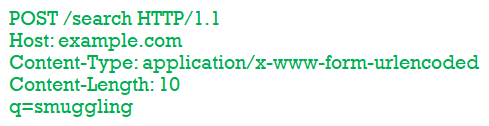
\includegraphics{images/Confirm_Request}
	\caption{Confirm - Target Request}
	\label{fig:Confirm_Request}
\end{figure}
If the target request looks as in figure \ref{fig:Confirm_Request}, then two types of socket poisoning are possible:
\begin{itemize}
	\item \textbf{CL.TE : } The request created for CL.TE poisoning is basically aiming to force a 404 response to the follow-up victim request. Figure \ref{fig:Confirm-CL.TE Poisoning}  
	\begin{figure}
		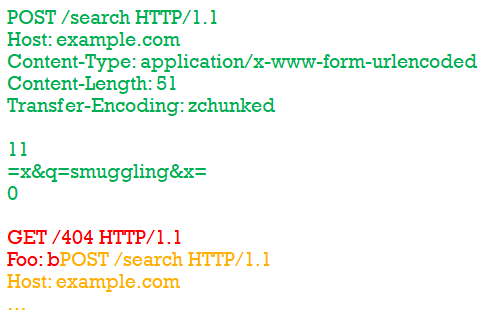
\includegraphics{images/Confirm_CL.TE}
		\caption{Confirm - CL.TE Poisoning}
		\label{fig:Confirm-CL.TE Poisoning}
	\end{figure}
	\item \textbf{TE.CL : } This is similar to CL.TE but the attacker needs to specify all the headers and ensure that the length of the malicious prefix is larger than the body. Figure \ref{fig:Confirm-TE.CL Poisoning}
	\begin{figure}
		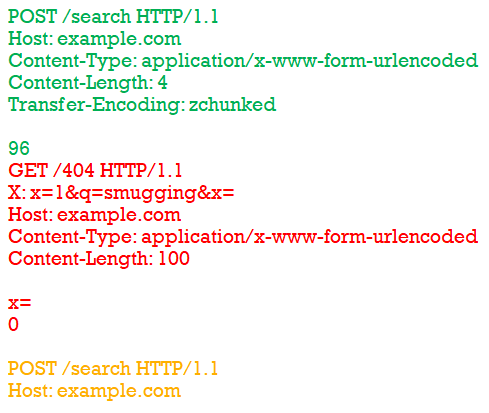
\includegraphics{images/Confirm_TE.CL}
		\caption{Confirm - TE.CL Poisoning}
		\label{fig:Confirm-TE.CL Poisoning}
	\end{figure}
\end{itemize}

\section{Explore}
Once we have established the fact that a target system is vulnerable for request smuggling attacks and the servers can be poisoned, we have to explore the ways in which an attack can be carried out. Explore phase aims to gather sensitive information which will help in attacking the target system. \\
There are several HTTP request headers such as \textsc{X-Forwarded-Host} and \textsc{X-Forwarded-For} that are often re-written by the frontend servers while transmitting the request. Though we try to change these headers manually, the frontend still re-writes these headers. This kind of configuration usually makes it difficult to by-pass the re-writes because the smuggled request may be missing these headers and can cause the system to exhibit unexpected behaviour. \\
One method to navigate across such header re-writes is to gradually gain visibility into these hidden headers by sending numerous investigative requests, observing the responses and further modifying the requests everytime before re-sending. This method is followed until the response reveals some information about the hidden headers, which we can use for our advantage. Once the hidden headers are revealed, we can modify our request to include these headers and further carryout attacks on the system. 
\subsection{Case Study for \textit{Explore} phase}
One simple example (as referenced from \cite{b6}) to demonstrate this is to explore a page in the target application which reflects a POST parameter. The smuggled request is modified accordingly by placing the reflected parameter at the last and increasing the \textsc{Content-length}. The modified request can now be smuggled. Figure \ref{fig:Explore_Request} shows one such example request.\\ 
\begin{figure}
	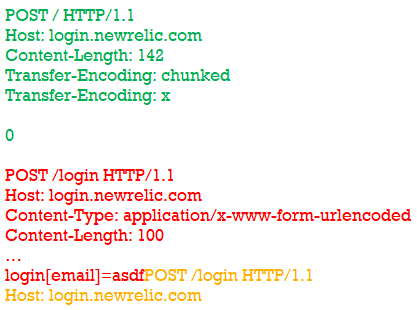
\includegraphics{images/Explore_Request}
	\caption{Explore - Request}
	\label{fig:Explore_Request}
\end{figure}
The follow-up request will be re-written by the frontend server before it encounters the $login[email]$ parameter. When the response is received, all the internal headers are revealed. 
The response to the request in figure \ref{fig:Explore_Request} can be as follows:
\begin{verbatim}
Please ensure that your email and password are correct.
<input id="email" value="asdfPOST /login HTTP/1.1
Host: login.newrelic.com
X-Forwarded-For: 81.139.39.150
X-Forwarded-Proto: https
X-TLS-Bits: 128
X-TLS-Cipher: ECDHE-RSA-AES128-GCM-SHA256
X-TLS-Version: TLSv1.2
x-nr-external-service: external
\end{verbatim}
Increasing the \textsc{Content-Length} header can reveal more and more information, until the entire victim request is parsed. 

\section{Store}
Once we explore the possible methods of poisoning the servers, we have two possibilities. One is to attack the victim or to store their data. In the store phase, we mainly aim to store the data revealed by the response to a victim's request. Once the server is poisoned with the malicious prefix we introduce, it gets appended to the next request. If a normal user (victim) sends this next request, their data can be stored and then we can make the application reveal their sensitive information. \\
For this method to work, the application needs to support some kind of data storage. If this is supported, the malicious prefix we send can be carefully crafted to contain a storage request. When this is appended to victim's request, it is possible to force the application to store the victim's information such as cookies/headers. 
\subsection{Case Study for \textit{Store} phase}
Figure \ref{fig:Store_Request} referenced from \cite{b6} demonstrates an example of storing victim's information.
\begin{figure}
	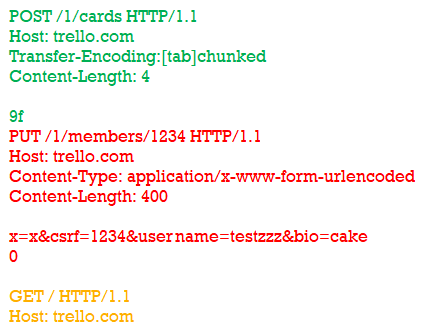
\includegraphics{images/Store_Request}
	\caption{Store - Request}
	\label{fig:Store_Request}
\end{figure}
The malicious prefix was crafted to target the Trello's profile-edit endpoint and was designed to store a victim's information on a test account in Trello.\\
\begin{figure}
	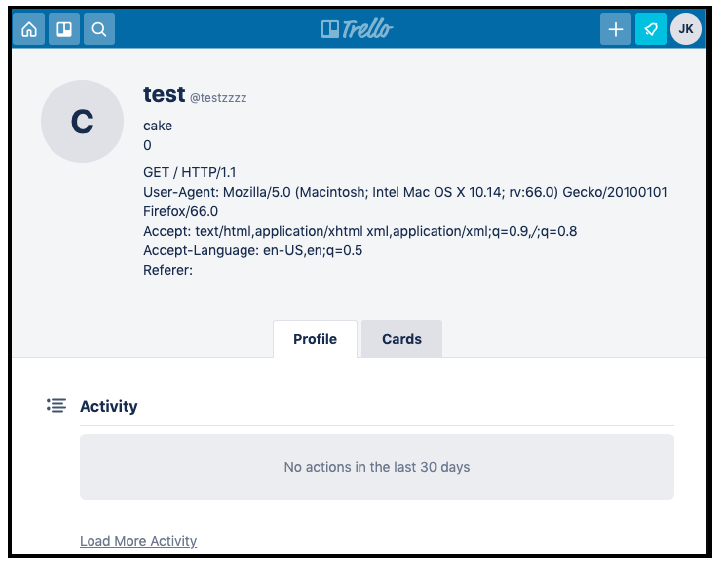
\includegraphics[width=14cm]{images/Store_Response}
	\caption{Store - Response}
	\label{fig:Store_Response}
\end{figure}
When the prefix got appended to the victim's request, their cookies and headers were routed and displayed in the test account. See figure \ref{fig:Store_Response} (Referenced from \cite{b6})\\

\section{Attack}
After exploring the poisoning options, another further option is to directly carry out the attack on the victims by triggering a harmful response. \\
Two primary methods for attacks are :
\begin{itemize}
	\item Trigger harmful response : Send malicious prefix that can 'attack', wait for the victim's request to get appended and then trigger harmful response. 
	\item Web-cache poisoning : Send both 'attack' and 'victim' request and then expect the response to be stored in a web cache. When any other user hits the same url, the web cache will serve the harmful response to all those users. 
\end{itemize}

\subsection{Attack methods}
Several attack methods can be employed and I intend to provide a very brief introduction to each of these methods:
\subsubsection{Upgrading XSS}
Cross-site Scripting(XSS) \cite{b11} enables an attacker to inject malicious scripts on the server. Upgrading XSS method uses request smuggling to rain mass havoc using XSS. Server response containing XSS are sent to numerous random users active on the website. This can exploit the victims in mass and can reveal authentication and cookie information of those victims.  
\subsubsection{Grasping the DOM}
If the victim's DOM \cite{b20} contains an open redirect, it can be chained with request smuggling and can be controlled to decieve the server to redirect the victim to an address that we specify.  
\subsubsection{CDN Chaining}
Many of the websites use several layers of CDNs \cite{b12} and reverse proxies \cite{b13}. Even though it is difficult to attack such websites, this setup also gives increased opportunities for desynchronization and request smuggling.
\subsubsection{Web Cache Poisoning}
Request smuggling can be used in combination with Web Cache Poisoning \cite{b14} to send malicious responses to multiple users. A poisoned request can be used to contaminate the web cache and any users whose request hits the web cache will be served with the malicious responses. \\

In addition to these attack methods, several other methods such as Web Cache Deception can also be used. 

\chapter{Defence against HTTP Desync Attacks}
\textit{Note to the supervisor : Will discuss about the case studies which the author has explained}



\section{Introduction}

If an attacker is able to snoop in on the data being exchanged, it can be used for malicious purposes. It can contain personal information of a person or an organisation, confidential data of goverments and organisations, financial data and so on.\\

HTTP has been constantly improved and has become an important protocol to secure the data that is transmitted over the internet. However, as the growth of internet increases the need for securing these data transfers also increases with it.\\

\section{Background}
\begin{itemize}
	\item HTTP\cite{b1} : 
	\item HTTP 1.1 :
	\item HTTP Headers :
\end{itemize}
\section{Problem Statement}
\section{Approach}
\section{Case Studies}
\section{Evaluation}
\section{Advantages and Disadvantages}
\section{Future Work}
\section{Conclusion}
\begin{thebibliography}{00}
	\bibitem{b1} https://tools.ietf.org/html/rfc7231 
	
\end{thebibliography}	

\end{document}
